\chapter{服务监控与应急措施优化}
在本论文的第三章和第四章分别对应用性能方面和数据库方面进行了优化,在系统优化的过程中,除了提升应用性能和数据库性能之外,对于服务器中运行的服务进行监控检查和报警,并且能够实现自动化的Failover也是系统优化的重点,本章将对于目前项目开发过程中使用的工具、软件设计开发相应的监控脚本,并且探索在服务监控过程中的报警和故障恢复模式\cite{刘雄辉2007服务器监控管理}。
\label{cha:Monitor}
\section{阿里云云监控应用}
云监控(CloudMonitor) 是一项针对阿里云资源和互联网应用进行监控的服务。云监控服务可用于收集获取阿里云资源的监控指标,探测互联网服务可用性,以及针对指标设置警报。由于本项目的所有服务器均为阿里云服务器,所以一部分的监控可以通过配置阿里云的云监控来实施。通过云监控服务能够监控云服务器 ECS、云数据库 RDS 和负载均衡等各种阿里云服务资源,同时也能够通过 HTTP,ICMP 等通用网络协议监控互联网应用的可用性。

在监控配置之前,需要对目前阿里云资源进行统计,如表~\ref{tab:aliyun-resources}所示:

\begin{longtable}[c]{c*{2}{c}}
\caption{项目阿里云资源整理}\label{tab:aliyun-resources}\\
\toprule[1.5pt]
{\heiti 资源类别} & \multicolumn{1}{c}{\heiti 资源实例}  & {\heiti 资源介绍} \\\midrule[1pt]
\endfirsthead
\multicolumn{3}{c}{续表~\thetable\hskip1em 项目阿里云资源整理}\\
\toprule[1.5pt]
{\heiti 资源类别} & \multicolumn{1}{c}{\heiti 资源实例}  & {\heiti 资源介绍} \\\midrule[1pt]
\endhead
\hline
\multicolumn{3}{r}{续下页}
\endfoot
\endlastfoot
\multirow{5}*{站点} &  生产环境地址 & 生产环境应用的负载均衡入口地址  \\
                        &  测试环境地址 & 测试环境应用的负载均衡入口地址  \\
                        &  主数据库地址 & 生产环境主数据库的访问地址和端口  \\
                        &  从数据库地址 & 生产环境从数据库的访问地址和端口  \\
                        &  Couchbase地址  & 生产环境Couchbase入口地址\\
\hline
\multirow{5}*{云服务器ECS}  &  APP1 & WEB应用服务器,提供WEB应用服务  \\
                        &  APP2 & WEB应用服务器,提供WEB应用服务  \\
                        &  DB1 & 主数据库服务器,WEB请求的主服务器  \\
                        &  DB2 & 从数据库服务器,同DB1主从复制,DB1出现问题时切换为主数据库  \\
                        &  TEST & 测试服务器,提供测试环境相关的服务  \\
\hline
\multirow{3}*{负载均衡}  &  prod & 生产环境WEB应用负载均衡  \\
                        &  dbslb & 生产环境数据库负载均衡  \\
                        &  test & 测试环境负载均衡  \\
\multirow{3}*{CDN}  &  web & WEB应用访问域名  \\
                    &  img & 图片服务器域名  \\
                    &  fileserver & 文档服务器域名  \\
\bottomrule[1.5pt]
\end{longtable}

为了保证各个阿里云资源的正常使用,通过阿里云的云监控配置各服务的监控项,并且增加报警联系人,在监控到问题的时候能够通过短信或邮件的方式及时通知运维人员,以便在短时间内解决问题。
\begin{enumerate}
\item 站点监控

站点监控通过HTTP协议和TCP协议根据设置的监控频率去检测各个站点的访问时间,以此来判断站点是否正常。

对于生产环境的WEB应用、测试环境的WEB应用以及生产环境的Couchbase,通过HTTP协议去访问对应的地址,对于主从数据库,通过TCP去测试数据库的链接是否正常。

监控的状态如图~\ref{fig:aliyun1}所示:
\begin{figure}[H] % use float package if you want it here
  \centering
  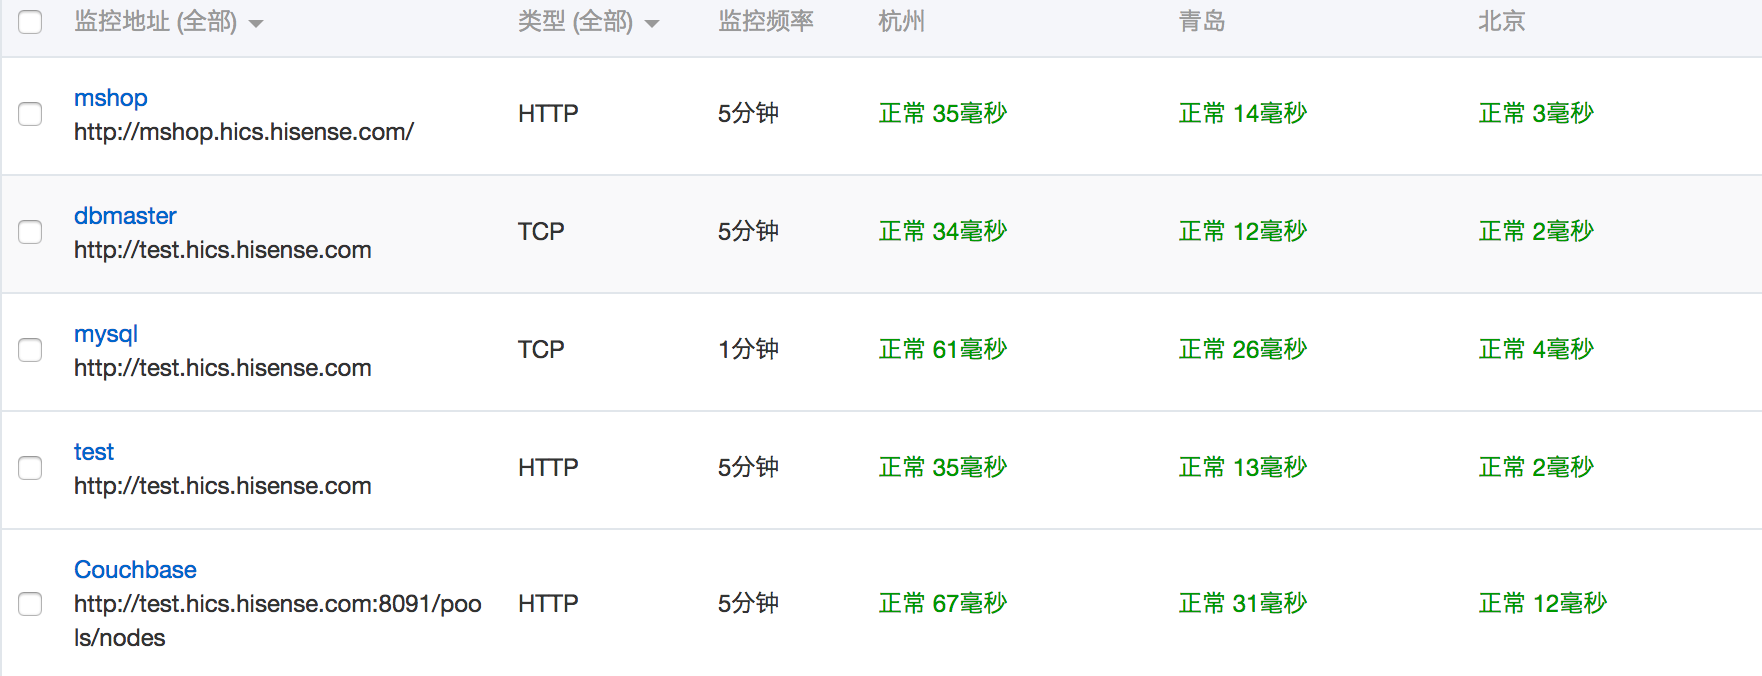
\includegraphics[width=6in]{chap05/aliyun1}
  \caption{站点监控状态图}
  \label{fig:aliyun1}
\end{figure}

\item 云服务器监控

云服务器的监控则通过安装在服务器中的阿里云监控插件获取云服务器的状态,对于所有的云服务监控的规则都是一样的,均为CPU使用率、内存使用率和磁盘使用率三个方面,监控的具体规则如表~\ref{tab:aliyun-ecs}所示:
\begin{table}[H]
  \centering
  \begin{minipage}[t]{0.8\linewidth} % 如果想在表格中使用脚注,minipage是个不错的办法
  \caption[阿里云监控]{云服务器监控规则}
  \label{tab:aliyun-ecs}
    \begin{tabularx}{\linewidth}{lX}
      \toprule[1.5pt]
      {\heiti 监控项} & {\heiti 监控描述}\\\midrule[1pt]
        CPU使用率 & 5分钟 CPU使用率 平均值>85\% 则报警\\
        内存使用率 & 5分钟 内存使用率 最大值>95\% 则报警\\
        磁盘使用率 & 5分钟 磁盘使用率 平均值>70\% 则报警\\
      \bottomrule[1.5pt]
    \end{tabularx}
  \end{minipage}
\end{table}

\item 负载均衡监控
负载均衡主要是监控负载均衡内的各个服务器的监控状态以及负载均衡的带宽状态,当负载均衡出现异常时,可以通知报警联系人及时作出应对。
\begin{itemize}
\item 生产环境应用负载均衡监控规则
\begin{table}[H]
  \centering
  \begin{minipage}[t]{0.8\linewidth} % 如果想在表格中使用脚注,minipage是个不错的办法
  \caption[阿里云监控]{生产环境应用负载均衡监控规则}
  \label{tab:aliyun-slb1}
    \begin{tabularx}{\linewidth}{lX}
      \toprule[1.5pt]
      {\heiti 监控项} & {\heiti 监控描述}\\\midrule[1pt]
        流出带宽&5分钟 流出带宽 平均值>3M/s 则报警\\
        流入带宽&5分钟 流入带宽 平均值>3M/s 则报警\\
        后端异常ECS实例数&1分钟 后端异常ECS实例数 平均值>0个 则报警\\
      \bottomrule[1.5pt]
    \end{tabularx}
  \end{minipage}
\end{table}
\item 生产环境数据库负载均衡监控规则
\begin{table}[H]
  \centering
  \begin{minipage}[t]{0.8\linewidth} % 如果想在表格中使用脚注,minipage是个不错的办法
  \caption[阿里云监控]{生产环境数据库负载均衡监控规则}
  \label{tab:aliyun-slb2}
    \begin{tabularx}{\linewidth}{lX}
      \toprule[1.5pt]
      {\heiti 监控项} & {\heiti 监控描述}\\\midrule[1pt]
        后端健康ECS实例数&1分钟 后端健康ECS实例数 平均值<1个 则报警\\
      \bottomrule[1.5pt]
    \end{tabularx}
  \end{minipage}
\end{table}
\item 测试环境负载均衡监控规则
\begin{table}[H]
  \centering
  \begin{minipage}[t]{0.8\linewidth} % 如果想在表格中使用脚注,minipage是个不错的办法
  \caption[阿里云监控]{测试环境负载均衡监控规则}
  \label{tab:aliyun-slb3}
    \begin{tabularx}{\linewidth}{lX}
      \toprule[1.5pt]
      {\heiti 监控项} & {\heiti 监控描述}\\\midrule[1pt]
        流出带宽&5分钟 流出带宽 平均值>3M/s 则报警\\
        流入带宽&5分钟 流入带宽 平均值>3M/s 则报警\\
        后端异常ECS实例数&1分钟 后端异常ECS实例数 平均值>0个 则报警\\
      \bottomrule[1.5pt]
    \end{tabularx}
  \end{minipage}
\end{table}
\end{itemize}
\item CDN监控
CDN监控时通过监控每一个域名的流量状态来判断应用的访问是否正常,当遇到DDos攻击时,CDN的流量会出现明显异常,通过监控这些异常,及时向运维用户报警,在很大程度上可以减少CDN流量的损失和降低攻击的风险。

目前CDN监控的规则如表~\ref{tab:aliyun-cdn}所示:
\begin{table}[H]
  \centering
  \begin{minipage}[t]{0.8\linewidth} % 如果想在表格中使用脚注,minipage是个不错的办法
  \caption[阿里云监控]{CDN监控规则}
  \label{tab:aliyun-cdn}
    \begin{tabularx}{\linewidth}{lXX}
      \toprule[1.5pt]
      {\heiti 报警维度} & {\heiti 监控项} & {\heiti 监控描述}\\\midrule[1pt]
        fileserver&网络带宽峰值&5分钟 宽带峰值 平均值>4000000bit/s 则报警\\
        fileserver&公网下行流量&5分钟 公网网络出流量 求和值>100M/s 则报警\\
        img&网络带宽峰值&5分钟 宽带峰值 平均值>4000000bit/s 则报警\\
        web&网络带宽峰值&5分钟 宽带峰值 平均值>5000000bit/s 则报警\\
      \bottomrule[1.5pt]
    \end{tabularx}
  \end{minipage}
\end{table}
\end{enumerate}
\section{自定义服务监控}
虽然阿里云的云监控功能很完善,但是对于错误恢复和特殊需求的监控做的还相对不足,因此需要在本地的服务器中自己搭建监控的环境,以提升系统的稳定性。

\subsection{心跳监听}
为了保证监控系统的高可用性,需要在APP1和APP2两个应用服务器同时搭建监控系统,为了保证两套监控系统在同一时间只有一个监控系统在运行需要配置心跳监听,从监控节点通过心跳监听来监听主监控节点的运行状态,当主监控节点出现故障时,从监控节点运行监控进程,保证监控的正常\cite{巩天宁2012基于}。

Heartbeat是一款开源提供高可用(Highly-Available)服务的软件,通过Heartbeat可以将资源(IP及程序服务等资源)从一台已经故障的计算机快速转移到另一台可以正常运转的机器上继续提供服务,一般称之为高可用服务。在实际生产应用场景中,heartbeat的功能和keepalived有很多相同之处,但在生产中,对实际的业务应用也是有区别的。如:keepalived主要是控制ip的漂移,配置、应用简单,而heartbeat则不但可以控制ip漂移,更擅长对资源服务的控制,配置、应用比较复杂~\cite{郭绪晶2012服务器集群系统高可用模块设计与实现}。由于Heartbeat能够对资源服务进行控制,所以本论文使用Heartbeat作为心跳监听的工具。

在服务器中配置心跳监听的步骤主要有以下步骤:
\begin{enumerate}
\item 下载和安装Heartbeat软件

访问 http://www.linux-ha.org/wiki/Downloads 下载Heartbeat软件,解压完成后进入软件的目录中,执行以下命令完成安装:
\begin{lstlisting}[language=sh,numbers=none]
./bootstrap
#进入源码目录生成配置文件:
./ConfigureMe configure
#编译安装
make && make install
\end{lstlisting}
安装完成后出现下面的信息表示安装成功:
\begin{lstlisting}[numbers=none]
heartbeat configuration:
    Version                  = "3.0.6"
    Executables              = "/usr/sbin"
    Man pages                = "/usr/share/man"
    Libraries                = "/usr/lib64"
    Header files             = "/usr/include"
    Arch-independent files   = "/usr/share"
    Documentation files      = "/usr/share/doc/heartbeat"
    State information        = "/var"
    System configuration     = "/etc"
    Init (rc) scripts        = "/etc/rc.d/init.d"
    Init (rc) defaults       = "/etc/sysconfig"
    Use system LTDL          = "yes"
    HA group name            = "haclient"
    HA group id              = "987"
    HA user name             = "hacluster"
    HA user user id          = "991"
    Build dopd plugin        = "yes"
    Enable times kludge      = "yes"
    CC_WARNINGS              = " -Wall -Wmissing-prototypes -Wmissing-declarations -Wstrict-prototypes -Wdeclaration-after-statement -Wpointer-arith -Wwrite-strings -Wcast-qual -Wcast-align -Wbad-function-cast -Winline -Wmissing-format-attribute -Wformat=2 -Wformat-security -Wformat-nonliteral -Wno-long-long -Wno-strict-aliasing -Werror "
    Mangled CFLAGS           = "-g -O2  -Wall -Wmissing-prototypes -Wmissing-declarations -Wstrict-prototypes -Wdeclaration-after-statement -Wpointer-arith -Wwrite-strings -Wcast-qual -Wcast-align -Wbad-function-cast -Winline -Wmissing-format-attribute -Wformat=2 -Wformat-security -Wformat-nonliteral -Wno-long-long -Wno-strict-aliasing -Werror  -ggdb3 -funsigned-char"
    Libraries                = "-lbz2 -lz -lc -luuid -lrt -ldl  -lltdl"
    RPATH enabled            = "no"
    Distro-style RPMs        = "no"
Note: If you use the 'make install' method for installation you
    also need to adjust '/etc/passwd' and '/etc/group' manually.
\end{lstlisting}
\item 配置Heartbeat软件,实现两个服务器的心跳监听

heartbeat主要的配置文件有3个,分别是authkeys,ha.cf和haresources,authkeys配置文件主要配置节点之间的认证方式,ha.cf时主要的配置文件,主要配置节点信息、网络信息、监听频率等信息,haresources文件主要配置需要运行的程序或脚本。这里以app1/app2两节点为例,其IP分别是10.46.170.191/10.172.89.141,这里示例的配置文件为app1的,app2的参考app1配置即可。

ha.cf主配置文件配置如下:
\begin{lstlisting}[numbers=none]
# 日志路径
logfile /var/log/ha-log
# 日志级别,默认是用系统日志
#logfacility     local0
# 发送心跳报文的间隔,默认单位为秒,也可以使用500ms来代理500毫秒,等同于0.5。
keepalive 2
# 认为对方宕掉的间隔时间,超过这个时间,则认为对方已经宕掉。
deadtime 30
# 认为对方可能宕掉的间隔时间。
warntime 10
# 等待对方启动的最大时间,(超过这个时间会自动认为对方已经启动成功?)。
initdead 120
# 表示heartbeat广播/单播通讯使用的udp端口。
udpport 694
# 心跳所使用的网络接口。
bcast   eth0
# 单播通讯,对方网络接口及IP地址。
ucast eth0 10.172.89.141
# 表示当主节点(即提供资源/服务的节点)正常之后是否将资源/服务切换回来。
auto_failback on
# 看门狗定时器,如果节点一分钟内没有心跳,则重启节点。
#watchdog /dev/watchdog
# 就是heartbeat集群中的节点信息(节点的主机名: uname -n)。
node    app2
node    app1
\end{lstlisting}
在配置过程中将app1配置为主节点,当配置auto\_failback为off时,app1节点异常时app2会接管继续执行监控程序,app1节点恢复后也不会移交监控程序,当配置auto\_failback为on时,app1节点恢复后app2回将资源移交回app1.

authkeys主配置文件配置如下:
\begin{lstlisting}[numbers=none]
auth 2
#1 crc
2 sha1 mimaminishop
#3 md5 somewords
\end{lstlisting}
该文件为heartbeat的认证文件,该文件主要是用于集群中两个节点的认证,采用的算法和密钥(如果有的话)在集群中节点上必须相同,目前提供了3种算法:crc/md5/sha1。其中crc不能够提供认证,它只能够用于校验数据包是否损坏,而sha1/md5需要一个密钥来进行认证,从资源消耗的角度来讲,md5消耗的比较多,sha1次之,因此建议一般使用sha1算法。

可以看出,示例中使用的是sha1算法,如果要换用其他算法只需要修改auth指令后面的数字,然后取消相应行的注释即可。另外,该文件的属性必须为600,否则heartbeat启动将失败。

haresources主配置文件配置如下:
\begin{lstlisting}[numbers=none]
app1 system_monitor
\end{lstlisting}
这表示Heartbeat启动时会执行资源路径中的system\_monitor脚本,实现服务的监控。
\item 配置监控脚本,实现服务的监控。
\begin{lstlisting}[numbers=none]
#!/bin/bash
# 基本变量配置
MONITOR_LOG_PATH="/tmp/system_monitor.log"
MONITOR_PID='/tmp/system_monitor.lock'
mysql_heal_script="/opt/sh/mysql/mysql_health_stat.sh"
mysql_sync_script="/opt/sh/mysql/mysql_sync_stat.sh"
tomcat_heal_script="/opt/sh/ssh/tomcat_health_stat.sh"
heal_stat=1
sync_stat=1
CHECK_TIME='30s'
export sms_send_count=0
export sms_send_count_1=0
export sms_send_count_tomcat=0
function check_db_health (){
    source $mysql_heal_script
    if [ $? = 0 ] ;then
        echo "--[OK]Mysql health is OK" >> $MONITOR_LOG_PATH
    else
        echo "--[ERROR]Mysql health is ERROR" >> $MONITOR_LOG_PATH
    fi
}
function check_db_sync (){
    source $mysql_sync_script
    if [ $? = 0 ] ;then
        echo "--[OK]Mysql sync is OK" >> $MONITOR_LOG_PATH
    else
        echo "--[ERROR]Mysql sync is ERROR" >> $MONITOR_LOG_PATH
    fi
}
function check_tomcat_health (){
    source $tomcat_heal_script
    if [ $? = 0 ] ;then
        echo "--[OK]Tomcat health is OK" >> $MONITOR_LOG_PATH
    else
        echo "--[ERROR]Tomcat health is ERROR" >> $MONITOR_LOG_PATH
    fi
}
start(){
    echo "Starting system_monitor ..."
    if [ -f $MONITOR_PID ];then
        echo "system_monitor is already started!"
        exit 0
    fi
    while [ true ]; do
        mypid=$$
        echo $mypid > $MONITOR_PID
        echo '####'(date '+%Y-%m-%d %H:%M:%S')####' >> $MONITOR_LOG_PATH
        check_db_health
        check_db_sync
        check_tomcat_health
        sleep ${CHECK_TIME}
    done
}

stop(){
    if [ -f $MONITOR_PID ];then
        echo "Stopping system_monitor ..."
        kill (cat $MONITOR_PID)
        rm -f $MONITOR_PID
    else
        echo "system_monitor is already stopped!"
    fi
}

status(){
    if [ -f $MONITOR_PID ];then
        echo "system_monitor is Running!"
    else
        echo "system_monitor is stopped!"
    fi
}

case "$1" in
start)
    start
    ;;
stop)
    stop
    ;;
status)
    status
    ;;
restart)
    stop
    start
    ;;
*)
    echo $"Usage: $0 {start|stop|status|restart}"
    exit 2
esac
\end{lstlisting}
通过system\_monitor脚本,每30秒对脚本中的监控服务进行一次监听,如果有新的监控脚本,可以在该脚本中脚本的路径并完成相关配置。
\end{enumerate}

\subsection{Tomcat监控}
对于Tomcat的监控监控,主要通过Python中ssh库的SSHClient()对象的connect方法连接到远程服务器中,然后通过exec\_command函数在服务器端执行systemctl is-active tomcat.service命令来检测Tomcat服务的健康状态,并且将规定好的状态码返回到监控脚本中,如果检测到异常,则通过systemctl restart tomcat.service命令来重新启动Tomcat服务。
具体的监控和故障处理脚本可以通过附录~\ref{cha:Tomcathealth}和附录~\ref{cha:Tomcatfailover}来查看
\subsection{数据库监控}
对于数据库的监控主要包括数据库监控状态监测和数据库主从复制状态监控。
\begin{enumerate}
\item 数据库健康状态监控

对于数据库的健康状态,通过mysql命令访问服务器数据库执行show status命令来判断数据库是否运行正常,如果有数据返回则说明数据库运行正常,负责数据库健康状态出现问题,出现问题后通过调用短信发送命令向运维人员发送通知,健康监控脚本可以参考附录~\ref{cha:mysqlhealth}。
\item 数据库同步状态监控

对于数据的同步状态,通过执行show slave status命令来获取从库的状态,然后首先查看SQL和IO线程是否为YES状态,其次通过延迟来判断数据库复制的延迟是否过大,最后通过判断Master\_Log\_File和Relay\_Master\_Log\_File的值是否相等以及判断同步的偏移量Read\_master\_log\_Pos和Exec\_Master\_log\_pos 的值是否相等来判断同步的健康状态。

当数据库同步出现故障时通过发送短信通知运维人员进行处理。

数据库同步状态监控的脚本可以参考~\ref{cha:mysqlsync}
\end{enumerate}
\section{短信通知}
在以前,当服务出现问题时无法及时的通知到运维人员,直到运维人员巡检活着应用的访问出现问题时运维人员才会发现故障,而现在有了监控的脚本,那么尽快的通知运维人员就是需要解决的一个主要问题。通知时效性最高的就是短信通知,因此在服务器中开发一个能够发送短信程序就显得非常重要\cite{陈泰伟2007基于短信平台的服务器监控系统关键技术探讨}。

为了实现短信的发送,首先需要选择和注册一个短信平台,由于云通讯平台短信发送的时间低于五秒,且支持自定义短信模版的功能,以及支持API的特点,本论文选择云通讯作为系统的短信发送应用。

其次,需要在服务中安装SDK,同时开发短信发送脚本调用SDK实现短信的发送,短信发送脚本如下所示:

\begin{lstlisting}[numbers=none]
# -*- coding: UTF-8 -*-
from CCPRestSDK import REST
import ConfigParser
import re
import sys
# 基本参数配置
# 主账号
accountSid= '主账户Id';
# 主账号Token
accountToken= '主账号验证token';
# 应用ID
appId='应用标识,每个创建的应用都对应唯一的id标识';
# 请求地址
serverIP='app.cloopen.com';
# 请求端口
serverPort='8883';
# REST版本号
softVersion='2013-12-26';
# 发送函数
def sendTemplateSMS(to,datas,tempId):
    rest = REST(serverIP,serverPort,softVersion)
    rest.setAccount(accountSid,accountToken)
    rest.setAppId(appId)
    result = rest.sendTemplateSMS(to,datas,tempId)
    for k,v in result.iteritems():
        if k=='templateSMS' :
                for k,s in v.iteritems():
                    print '%s:%s' % (k, s)
        else:
            print '%s:%s' % (k, v)
# 主函数
def main():
    if len(sys.argv) == 4:
        # 编码调整
        reload(sys)
        sys.setdefaultencoding('utf-8')
        # 变量处理
        to=sys.argv[1]
        tempId=sys.argv[2]
        datas=re.split('-',sys.argv[3])
        sendTemplateSMS(to,datas,tempId)
        sys.exit(0)
    else:
        print "参数错误"
        sys.exit(1)
if __name__=='__main__':
    main()
\end{lstlisting}
在脚本中,首先需要根据自己注册的账户获取账户ID和验证Token,然后获取自己创建的应用的ID,完成基础的配置和认证。
在执行脚本时,通过SendTemplateSMS.py phone tempID content命令来发送短信,其中phone为接受短信的一个或者一组手机号,tempID为自己设计的短信模版对于的ID,contenet为短信的发送内容。
\section{日志备份}
在Tomcat的运行过程中,随着用户的访问,每天都会产生大量的访问日志和请求日志,随时时间的增加,日志的数量和空间占用会越来越大,为了解决日志的空间占用问题同时保证日志的存储以便后期进行日志分析,需要设计开发日志备份脚本。主要的需求为:
\begin{itemize}
\item 每个月的1号会压缩上一个月的日志文件到压缩文件中
\item 每个月清理超过三个月的日志
\item 每个月压缩的日志上传到阿里云归档存储中进行备份
\end{itemize}
针对以上需求,开发的归档存储上传脚本为:
\begin{lstlisting}[numbers=none]
#!/usr/bin/python2.7
# -*- coding: utf-8 -*-
from oas.oas_api import OASAPI
from oas.ease.vault import Vault
import sys
def main():
    if len(sys.argv) == 4:
        # 变量处理
        vault_name=sys.argv[1]
        file_path=sys.argv[2]
        file_desc=sys.argv[3]
        # 创建OASAPI对象
        api = OASAPI('cn-beijing.oas-internal.aliyuncs.com','AccessKeyId', 'AccessKeySecret')
        # 获取vault
        vault = Vault.get_vault_by_name(api,vault_name)
        # 上传后获取archiveid
        archive_id = vault.upload_archive(file_path,file_desc)
        print archive_id
        sys.exit(0)
    else:
        print "参数错误"
        sys.exit(1)
if __name__=='__main__':
    main()
\end{lstlisting}
通过oas库中oas\_api方法链接获取到OAS对象,通过对象的upload\_archive方法上传备份的日志文件。

开发的日志备份脚本可以参考附录~\ref{cha:Tomcatlog},脚本中首先通过匹配不同类型的日志名称来将日志文件分类压缩,然后通过执行OAS上传脚本上传压缩后的日志文件,上传完成后删除未压缩的日志文件。

日志备份脚本开发完成后,为了保证脚本每个月运行一次,需要修改crontab的配置文件,增加:
\begin{lstlisting}[numbers=none]
0 3 1 * * /opt/sh/Prod_tomcat_log_bak.sh
\end{lstlisting}
设置脚本执行时间为每个月1号的凌晨3点。
%\section{DockerAPI操作}
%\section{阿里云API优化}
\label{cha:Monitor-aliyun}
\section{本章总结}
本章主要对服务器层级的服务器监控措施和应急措施的优化策略研究,主要包括基于阿里云平台的自有监控和通知方案设计、个人开发的服务监控方案设计、短信通知脚本开发以及日志定期备份脚本开发等内容,通过以上的监控和优化措施的开发,在最大程度上保证服务器的正常运行、服务的正常运行、服务故障的自动恢复以及服务故障的通知,降低运维人员的时间成本,努力提升系统的稳定性。